%% IEEE Software — Revised v2
%% Authors: Florin Olariu, Lenuta Alboaie
%% Template: IEEEtran v1.8b, compsoc journal mode
\documentclass[10pt,journal,compsoc]{IEEEtran}

% ---------- packages ----------
\usepackage{cite}
\usepackage{amsmath,amssymb}
\usepackage{graphicx}
\usepackage{xcolor}
\usepackage{booktabs}
\usepackage{array}
\usepackage{url}
\usepackage{hyperref}
\usepackage{tikz}
\usetikzlibrary{shapes.geometric, arrows.meta, positioning, fit,
                backgrounds, decorations.pathreplacing}
\usepackage{balance}
\usepackage{listings}
\lstset{basicstyle=\small\ttfamily,breaklines=true,frame=none,
        keywordstyle=\color{blue!70!black},commentstyle=\color{gray}}

% ---------- title block ----------
\title{From Monolith to Cloud: An Agentic AI Pipeline\\
       for .NET Microservices Migration}

\author{Florin~Olariu~and~Lenuta~Alboaie%
  \IEEEcompsocitemizethanks{%
    \IEEEcompsocthanksitem F.~Olariu is with the Faculty of Computer
      Science, Alexandru Ioan Cuza University of Ia\c{s}i, Romania,
      and with Suvoda LLC. E-mail: \url{folariu@suvoda.com}
    \IEEEcompsocthanksitem L.~Alboaie is with the Faculty of Computer
      Science, Alexandru Ioan Cuza University of Ia\c{s}i, Romania.
  }%
}

\markboth{IEEE Software,~Vol.~XX,~No.~X,~2026}%
         {Olariu \& Alboaie: From Monolith to Cloud}

\IEEEtitleabstractindextext{%
% ---------- abstract ----------
\begin{abstract}
Migrating a monolithic application to cloud-deployed microservices is
one of the most consequential and labour-intensive transformations in
enterprise software engineering.  We report a complete, end-to-end
migration of \textit{PetRescue}, a .NET~10 ASP.NET~Core monolith, to
independently deployable microservices running on Oracle Cloud
Infrastructure—executed and validated using a ten-skill agentic AI
pipeline built on Claude~Code.
The migration journey spans four artefacts: the original monolith
(Slice~1), an expert hand-crafted microservices decomposition (Slice~2)
produced independently as a reference, an AI-generated decomposition
produced by the pipeline (Slice~1~Refactored), and a Terraform
configuration for cloud provisioning (Slice~3).
The AI-generated decomposition—produced in approximately five minutes
compared to one developer-day for the expert manual migration—matches
the expert reference across all twenty pre-defined structural
dimensions.  The same pipeline adds a new feature identically to both
codebases in a complete quality-gated cycle of approximately
30~minutes, including automated detection and remediation of three
critical and four high-severity security findings before the commit
is allowed.  The pipeline then provisions an OCI Ampere~A1.Flex ARM64
instance via Terraform with a cloud-init bootstrap.
The pipeline is grounded in three design principles—skill atomicity,
artefact-mediated state, and gated autonomy—that make it auditable,
safe to use in CI/CD contexts, and portable across projects.
All four artefacts are publicly available on GitHub.
\end{abstract}

% ---------- keywords ----------
\begin{IEEEkeywords}
cloud migration, microservices, monolith decomposition, agentic AI,
LLM agents, SDLC automation, DevSecOps, Infrastructure as Code,
.NET, Oracle Cloud Infrastructure
\end{IEEEkeywords}
}

\begin{document}
\maketitle
\IEEEdisplaynontitleabstractindextext
\IEEEpeerreviewmaketitle

% ============================================================
%  ACTIONABLE INSIGHTS  (required by IEEE Software)
% ============================================================
\begin{IEEEcompsocoutcaseinitial}A\end{IEEEcompsocoutcaseinitial}
\textbf{Actionable Insights}
\begin{itemize}
  \item An agentic AI pipeline—ten slash-commands backed by Claude~Code
        skill scripts—can execute a complete .NET monolith-to-cloud
        migration: decomposition, feature addition, security remediation,
        and Terraform deployment, with human-readable checkpoints at
        every stage.
  \item The \texttt{/refactor} skill reproduces an expert
        architect's decomposition decisions (20/20 structural
        dimensions) in approximately \textbf{5~minutes}—compared to
        \textbf{one developer-day} for the hand-crafted reference—
        while independently inferring security patterns the skill
        prompt does not enumerate.
  \item Chaining \texttt{/check\_security} and \texttt{/fix} as hard
        preconditions of \texttt{/publish} prevents critical and
        high-severity vulnerabilities from ever reaching the repository,
        with no manual remediation required for the class of findings
        addressed.
\end{itemize}

% ============================================================
\section{Introduction}
\label{sec:intro}
% ============================================================

The migration of a monolithic application to cloud-native microservices
is one of the most consequential decisions a software organisation can
make, and also one of the most expensive to execute
well~\cite{newman2019monolith,taibi2017processes}.  Practitioners must
identify service boundaries, define inter-service contracts, replicate
cross-cutting concerns, and preserve all existing behaviour—while the
original system continues to evolve and while DevSecOps requirements
demand that no security debt be introduced in the process.

LLM-based coding assistants have demonstrated measurable productivity
gains on isolated, bounded tasks~\cite{peng2023copilot,
vaithilingam2022expectation}.  But a monolith-to-cloud migration is
not a collection of isolated tasks: it is a \emph{structured workflow}
whose stages are data-dependent, whose intermediate artefacts are
decisions (not just code), and whose correctness must be verified
before each downstream step.  No single LLM prompt can orchestrate
this reliably.  Recent agentic AI research—systems that combine
reasoning with action execution in an iterative
loop~\cite{yao2023react,wang2024agents}—offers a path forward, but
existing agentic SE benchmarks~\cite{jimenez2024swebench} target
narrow, single-issue tasks rather than full SDLC workflows.

This paper closes that gap with a complete, reproducible case study.
We describe the full migration of \textit{PetRescue}, a .NET~10
ASP.NET~Core monolith, executed by a ten-skill agentic pipeline and
deployed to Oracle Cloud Infrastructure.  The migration produces four
publicly available artefacts:

\begin{itemize}
  \item \textbf{Slice~1} — the original monolith, as the starting point.
  \item \textbf{Slice~2} — a hand-crafted microservices decomposition
        produced independently by the second author, serving as the
        expert reference.
  \item \textbf{Slice~1~Refactored} — an AI-generated decomposition
        produced by the pipeline's \texttt{/refactor} skill, compared
        against Slice~2 to validate decomposition quality.
  \item \textbf{Slice~3} — a Terraform configuration that provisions
        an OCI Ampere A1.Flex ARM64 virtual machine and deploys either
        slice via Docker Compose and cloud-init.
\end{itemize}

The pipeline is grounded in three design principles that determine
whether an agentic SDLC system is reliable rather than merely
impressive: \emph{skill atomicity} (each agent has one responsibility
and explicit file-level boundaries), \emph{artefact-mediated state}
(agents communicate through persistent Markdown files, not ephemeral
context), and \emph{gated autonomy} (downstream actions are blocked
until upstream quality criteria are formally satisfied).

We contribute:
\begin{enumerate}
  \item A complete end-to-end cloud migration of a real .NET monolith,
        executed by an agentic AI pipeline from source analysis through
        to a running OCI cloud service.
  \item Empirical validation that the AI-generated decomposition matches
        an expert reference across twenty pre-defined structural
        dimensions (20/20), and that the pipeline can add a new feature
        identically to both codebases.
  \item A \emph{reproducible pilot}: ten open-source Claude~Code skill
        scripts, four application repositories, and a Terraform
        configuration that any team can clone and run on their own
        .NET monolith without modification.  The skills are the
        reusable unit of contribution; PetRescue is the validation
        vehicle that demonstrates they produce correct, expert-quality
        results.
\end{enumerate}

% ============================================================
\section{Background and Related Work}
\label{sec:background}
% ============================================================

\subsection{Monolith-to-Microservices Migration}
Mazlami~et~al.~\cite{mazlami2017extraction} propose logical, semantic,
and contributor coupling strategies for partitioning a monolith into
candidate services.  Richardson~\cite{richardson2018patterns} codifies
the resulting architectural patterns.  Chen~\cite{chen2018devops}
empirically links microservice granularity to continuous-delivery lead
time.  Taibi~et~al.~\cite{taibi2017processes} interviewed 21
practitioners and identified boundary identification as the dominant
migration obstacle.  Evans~\cite{evans2003ddd} provides the theoretical
basis—domain-driven design and bounded contexts—that our
\texttt{/refactor} skill operationalises.  Our work complements this
body of literature by contributing the first end-to-end agentic pipeline
that executes the full migration, not only the decomposition step.

\subsection{Agentic AI Systems for Software Engineering}
Yao~et~al.'s ReAct~\cite{yao2023react} showed that interleaving LLM
reasoning traces with tool-call actions reduces hallucination and
improves performance on multi-hop tasks.
Wang~et~al.~\cite{wang2024agents} survey the broader landscape of
LLM-based autonomous agents, identifying memory, tool use, and
planning as the three architectural pillars.
SWE-bench~\cite{jimenez2024swebench} established that agentic systems
can resolve real GitHub issues; top agents at publication resolved
roughly 20–30\% of benchmark tasks, with failures concentrated on
multi-file, multi-step reasoning.

Our pipeline differs from these systems in two ways.
First, it targets a \emph{full SDLC workflow}—ten ordered stages with
data dependencies—rather than a single task.  Second, it implements
\emph{gated autonomy}: the pipeline halts at defined checkpoints,
writes a human-readable gate document, and refuses to proceed until
the gate is cleared.  This makes the pipeline auditable and safe for
enterprise CI/CD contexts, properties that continuous-loop agents do
not currently offer.

\subsection{LLM-Assisted Code Review and Security}
Hou~et~al.'s review~\cite{hou2024llmse} finds code generation, program
repair, and test synthesis as the LLM tasks with the strongest and most
consistent results.  DevSecOps research~\cite{mohan2021devsecops}
advocates shifting security left into the development loop.  Our
pipeline addresses both: it generates code, repairs security findings,
generates tests, and gates the commit on security criteria—all within a
single coherent workflow.

% ============================================================
\section{The Agentic Migration Pipeline}
\label{sec:pipeline}
% ============================================================

\begin{figure*}[!t]
  \centering
  % Pipeline diagram — 10 skills + Terraform deployment stage
% Compile with pdflatex (tikz, shapes.geometric, arrows.meta, positioning, backgrounds)
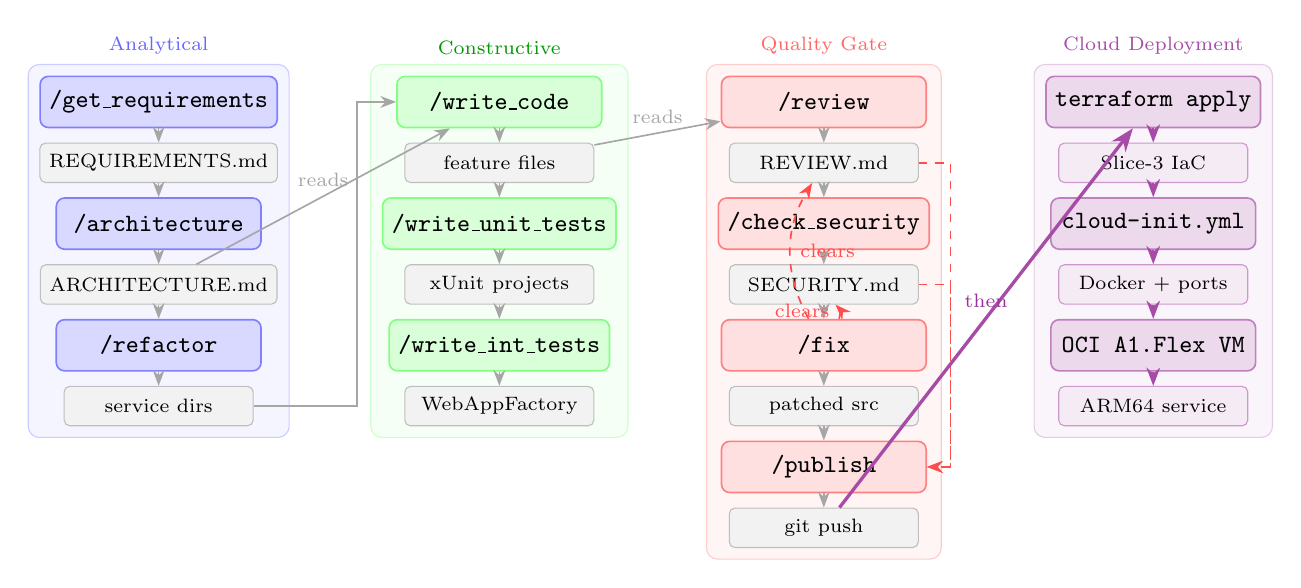
\begin{tikzpicture}[
  skill/.style = {
    rectangle, rounded corners=3pt,
    minimum width=2.6cm, minimum height=0.65cm,
    font=\small\ttfamily, text centered,
    line width=0.6pt
  },
  artefact/.style = {
    rectangle, rounded corners=2pt,
    minimum width=2.4cm, minimum height=0.5cm,
    font=\scriptsize, text centered,
    fill=gray!10, draw=gray!50, line width=0.4pt
  },
  cloud/.style = {
    rectangle, rounded corners=3pt,
    minimum width=2.6cm, minimum height=0.65cm,
    font=\small\ttfamily, text centered,
    fill=violet!15, draw=violet!50, line width=0.6pt
  },
  cloudout/.style = {
    rectangle, rounded corners=2pt,
    minimum width=2.4cm, minimum height=0.5cm,
    font=\scriptsize, text centered,
    fill=violet!8, draw=violet!40, line width=0.4pt
  },
  arrow/.style  = {-Stealth, line width=0.6pt, gray!70},
  gate/.style   = {arrow, red!70, dashed},
  deploy/.style = {-Stealth, line width=0.8pt, violet!70},
  node distance = 0.35cm
]

% ---- colour definitions ----
\colorlet{analyticfill}{blue!15}
\colorlet{analyticborder}{blue!50}
\colorlet{constructfill}{green!15}
\colorlet{constructborder}{green!50}
\colorlet{gatefill}{red!12}
\colorlet{gateborder}{red!50}

% ===========================
% COLUMN 1 : analytical skills
% ===========================
\node[skill, fill=analyticfill, draw=analyticborder]
  (req)  {/get\_requirements};
\node[artefact, below=0.18cm of req]
  (reqout) {REQUIREMENTS.md};

\node[skill, fill=analyticfill, draw=analyticborder,
      below=0.18cm of reqout]
  (arch)  {/architecture};
\node[artefact, below=0.18cm of arch]
  (archout) {ARCHITECTURE.md};

\node[skill, fill=analyticfill, draw=analyticborder,
      below=0.18cm of archout]
  (ref)  {/refactor};
\node[artefact, below=0.18cm of ref]
  (refout) {service dirs};

% ===========================
% COLUMN 2 : constructive skills
% ===========================
\node[skill, fill=constructfill, draw=constructborder,
      right=1.5cm of req]
  (wc)  {/write\_code};
\node[artefact, below=0.18cm of wc]
  (wcout) {feature files};

\node[skill, fill=constructfill, draw=constructborder,
      below=0.18cm of wcout]
  (wu)  {/write\_unit\_tests};
\node[artefact, below=0.18cm of wu]
  (wuout) {xUnit projects};

\node[skill, fill=constructfill, draw=constructborder,
      below=0.18cm of wuout]
  (wi)  {/write\_int\_tests};
\node[artefact, below=0.18cm of wi]
  (wiout) {WebAppFactory};

% ===========================
% COLUMN 3 : quality-gate skills
% ===========================
\node[skill, fill=gatefill, draw=gateborder,
      right=1.5cm of wc]
  (rv)  {/review};
\node[artefact, below=0.18cm of rv]
  (rvout) {REVIEW.md};

\node[skill, fill=gatefill, draw=gateborder,
      below=0.18cm of rvout]
  (sec)  {/check\_security};
\node[artefact, below=0.18cm of sec]
  (secout) {SECURITY.md};

\node[skill, fill=gatefill, draw=gateborder,
      below=0.18cm of secout]
  (fix)  {/fix};
\node[artefact, below=0.18cm of fix]
  (fixout) {patched src};

\node[skill, fill=gatefill, draw=gateborder,
      below=0.18cm of fixout]
  (pub)  {/publish};
\node[artefact, below=0.18cm of pub]
  (pubout) {git push};

% ===========================
% COLUMN 4 : deployment stage (Terraform / OCI)
% ===========================
\node[cloud,
      right=1.5cm of rv]
  (tf)  {terraform apply};
\node[cloudout, below=0.18cm of tf]
  (tfout) {Slice-3 IaC};

\node[cloud,
      below=0.18cm of tfout]
  (ci)  {cloud-init.yml};
\node[cloudout, below=0.18cm of ci]
  (ciout) {Docker + ports};

\node[cloud,
      below=0.18cm of ciout]
  (vm)  {OCI A1.Flex VM};
\node[cloudout, below=0.18cm of vm]
  (vmout) {ARM64 service};

% ===========================
% ARROWS — within columns
% ===========================
\draw[arrow] (req)    -- (reqout);
\draw[arrow] (reqout) -- (arch);
\draw[arrow] (arch)   -- (archout);
\draw[arrow] (archout)-- (ref);
\draw[arrow] (ref)    -- (refout);

\draw[arrow] (wc)     -- (wcout);
\draw[arrow] (wcout)  -- (wu);
\draw[arrow] (wu)     -- (wuout);
\draw[arrow] (wuout)  -- (wi);
\draw[arrow] (wi)     -- (wiout);

\draw[arrow] (rv)     -- (rvout);
\draw[arrow] (rvout)  -- (sec);
\draw[arrow] (sec)    -- (secout);
\draw[arrow] (secout) -- (fix);
\draw[arrow] (fix)    -- (fixout);
\draw[arrow] (fixout) -- (pub);
\draw[arrow] (pub)    -- (pubout);

\draw[deploy] (tf)    -- (tfout);
\draw[deploy] (tfout) -- (ci);
\draw[deploy] (ci)    -- (ciout);
\draw[deploy] (ciout) -- (vm);
\draw[deploy] (vm)    -- (vmout);

% ===========================
% ARROWS — cross-column
% ===========================
% analytical → constructive
\draw[arrow] (archout) -- node[above,font=\scriptsize]{reads} (wc);
\draw[arrow] (refout)  -| ([xshift=-0.5cm]wc.west) -- (wc);

% constructive → gate
\draw[arrow] (wcout) -- node[above,font=\scriptsize]{reads} (rv);

% gate internal
\draw[gate, bend left=30]
  (fix) to node[right,font=\scriptsize,red!70]{clears} (rvout);
\draw[gate, bend right=30]
  (fix) to node[left,font=\scriptsize,red!70]{clears} (secout);

% gate check at /publish
\draw[gate] (rvout)  -| ([xshift=0.3cm]pub.east) -- (pub);
\draw[gate] (secout) -| ([xshift=0.3cm]pub.east) -- (pub);

% /publish git push → terraform apply (practitioner-run next step)
\draw[deploy, very thick]
  (pubout) -- node[above,font=\scriptsize,violet!80]{then} (tf);

% ===========================
% BACKGROUND BOXES
% ===========================
\begin{scope}[on background layer]
  \node[fit=(req)(reqout)(arch)(archout)(ref)(refout),
        fill=blue!4, draw=blue!20, rounded corners=4pt,
        inner sep=4pt,
        label={[font=\scriptsize,blue!60]above:Analytical}] {};
  \node[fit=(wc)(wcout)(wu)(wuout)(wi)(wiout),
        fill=green!4, draw=green!20, rounded corners=4pt,
        inner sep=4pt,
        label={[font=\scriptsize,green!60!black]above:Constructive}] {};
  \node[fit=(rv)(rvout)(sec)(secout)(fix)(fixout)(pub)(pubout),
        fill=red!4, draw=red!20, rounded corners=4pt,
        inner sep=4pt,
        label={[font=\scriptsize,red!60]above:Quality Gate}] {};
  \node[fit=(tf)(tfout)(ci)(ciout)(vm)(vmout),
        fill=violet!4, draw=violet!20, rounded corners=4pt,
        inner sep=4pt,
        label={[font=\scriptsize,violet!70]above:Cloud Deployment}] {};
\end{scope}

\end{tikzpicture}

  \caption{The end-to-end agentic migration pipeline.
    Analytical skills (blue) write Markdown artefacts
    (\emph{artefact-mediated state}).
    Constructive skills (green) implement code from those artefacts
    alone (\emph{skill atomicity}).
    Quality-gate skills (red) enforce \emph{gated autonomy}:
    \texttt{/publish} blocks the commit until both gate documents
    are clear.
    The Cloud Deployment column (violet) completes the migration:
    after \texttt{/publish} pushes to GitHub, the practitioner runs
    \texttt{terraform apply} (Slice~3), which provisions an OCI
    Ampere A1.Flex ARM64 VM via \texttt{cloud-init.yaml} and starts
    the Docker Compose stack.  Both Slice~1~Refactored and Slice~2
    deploy via the same Terraform configuration because
    \texttt{/refactor} mandated identical port layouts in both.}
  \label{fig:pipeline}
\end{figure*}

Each skill is a directory containing a \texttt{SKILL.md} file that
Claude~Code~\cite{anthropic2024claude} loads as an extended system
prompt when the corresponding slash-command is entered.
Figure~\ref{fig:pipeline} shows the pipeline; Table~\ref{tab:skills}
summarises all ten skills with their inputs, outputs, and gate roles.

\subsection{Analytical Skills: Capturing Migration Intent}
\texttt{/get\_requirements} traverses the source tree—entities,
routes, EF~Core \texttt{DbContext} subclasses, environment-variable
toggles—and writes \texttt{REQUIREMENTS.md}: functional requirements,
API surface, data model, and NFRs.

\texttt{/architecture} reads \texttt{REQUIREMENTS.md} and writes
\texttt{ARCHITECTURE.md}: an ASCII service topology, per-service route
tables, inter-service dependency lists, and database ownership
assignments.  This document becomes the single authoritative
specification for all downstream skills; nothing that is not in
\texttt{ARCHITECTURE.md} is acted upon.

\texttt{/refactor} reads \texttt{ARCHITECTURE.md} and produces the
full microservices layout: four service directories
(\textit{Animals.Api}, \textit{Medical.Api}, \textit{Adopters.Api},
\textit{Gateway}), a shared contracts library with typed DTOs, a YARP
reverse-proxy configuration, schema-isolated
\texttt{appsettings.json} files using EF~Core
\texttt{HasDefaultSchema} with \texttt{Search~Path} overrides, and a
\texttt{docker-compose.yml} with \texttt{env\_file} references
rather than inline secrets.

\subsection{Constructive Skills: Extending the Migration}
\texttt{/write\_code <feature>} reads only \texttt{ARCHITECTURE.md}
to determine service ownership, then writes the DTO in the shared
library, the handler in the owning service, the gateway route, and
the compose wiring.  The intentional constraint—one input document,
no codebase context—is what makes the skill portable to codebases it
did not produce (demonstrated in Section~\ref{sec:eval-rq2}).

\texttt{/write\_unit\_tests} writes xUnit and Moq test projects, one
per service, following the Arrange-Act-Assert pattern with mocked
\texttt{DbContext} and typed-client substitutes.
\texttt{/write\_integration\_tests} writes WebApplicationFactory
fixtures with WireMock.Net stubs for cross-service HTTP calls and a
dedicated \texttt{docker-compose.test.yml}.

\subsection{Quality-Gate Skills: Enforcing Gated Autonomy}
\texttt{/review} writes \texttt{REVIEW.md} with findings at three
levels: \emph{blocking}, \emph{warning}, \emph{suggestion}.
\texttt{/check\_security} writes \texttt{SECURITY.md} with findings
at four levels: \emph{critical}, \emph{high}, \emph{medium},
\emph{low}.  The top tier of each document blocks publication.

\texttt{/fix} reads both documents and remediates every blocking and
critical/high finding in the source code, then marks them resolved.
Medium/low security issues and warnings remain visible but do not
block—preserving human judgement for trade-offs with no single correct
answer (e.g., TLS termination at the service vs.\ at a load balancer).

\texttt{/publish} performs a formal precondition check: it reads both
gate documents, scans for any unresolved blocking or critical/high
marker, and refuses to touch \texttt{git} if any are found.  On a
clean gate it stages only safe files (explicitly excluding
\texttt{.env} and \texttt{*.tfvars}), writes a conventional commit
message, and pushes to the remote.

\subsection{Cloud Deployment: Terraform on OCI}
After \texttt{/publish} commits the microservices code, the migration
is completed by a Terraform configuration (Slice~3) that provisions
cloud infrastructure without manual steps.

\texttt{main.tf} declares a Virtual Cloud Network, public subnet,
internet gateway, and an OCI Ampere~A1.Flex compute instance—an
ARM64 shape available on OCI's Always~Free tier at up to 4~OCPUs and
24~GB RAM, making the deployment fully reproducible at zero cost.
A \texttt{cloud-init.yaml} bootstrap script installs Docker Engine,
opens \texttt{iptables} INPUT rules for ports 5101 (Animals.Api),
5102 (Medical.Api), and 5103 (Adopters.Api), clones the target
application repository, and runs \texttt{docker~compose~up}.

Sensitive values—tenancy OCID and the SSH public key—live in
\texttt{terraform.tfvars}, which is excluded from version control
by \texttt{.gitignore}.  The \texttt{outputs.tf} block emits
\texttt{next\_steps\_slice1}, \texttt{next\_steps\_slice2}, and
\texttt{teardown} outputs, so running \texttt{terraform~apply}
delivers a ready-to-copy deployment command for either codebase.
The fact that both Slice~1~Refactored and Slice~2 are deployable
with the identical Terraform configuration—because \texttt{/refactor}
mandated the same port layout and \texttt{docker~compose} interface
in both—demonstrates that \emph{artefact-mediated state propagates
architectural decisions end-to-end}, from the \texttt{ARCHITECTURE.md}
document to the cloud.

\begin{table}[!t]
  \caption{Summary of the Ten Migration Skills}
  \label{tab:skills}
  \centering
  \small
  \setlength{\tabcolsep}{4pt}
  \begin{tabular}{@{}lllc@{}}
    \toprule
    \textbf{Skill} & \textbf{Reads} & \textbf{Writes} & \textbf{Gate?} \\
    \midrule
    \texttt{/get\_requirements}         & source tree       & REQUIREMENTS.md     & --     \\
    \texttt{/architecture}              & REQUIREMENTS.md   & ARCHITECTURE.md     & --     \\
    \texttt{/refactor}                  & ARCHITECTURE.md   & service dirs        & --     \\
    \texttt{/write\_code}               & ARCHITECTURE.md   & feature files       & --     \\
    \texttt{/write\_unit\_tests}        & source tree       & xUnit projects      & --     \\
    \texttt{/write\_integration\_tests} & source tree       & WebAppFactory tests & --     \\
    \texttt{/review}                    & source tree       & REVIEW.md           & writes \\
    \texttt{/check\_security}           & source tree       & SECURITY.md         & writes \\
    \texttt{/fix}                       & REVIEW + SECURITY & source + gate docs  & clears \\
    \texttt{/publish}                   & REVIEW + SECURITY & git commit + push   & checks \\
    \bottomrule
  \end{tabular}
\end{table}

% ============================================================
\section{Evaluation}
\label{sec:evaluation}
% ============================================================

\subsection{Migration Study Design}
The evaluation follows the full migration journey.  Slice~1 is the
original monolith—a single ASP.NET~Core process with five entities
and five performance anti-pattern scenarios (S1–S5, each with an
optimised toggle), measured under JMeter load with a CodeCarbon
energy sidecar.

Slice~2 is the expert reference: the second author independently
designed and built a four-service microservices decomposition of the
same monolith \emph{without any knowledge of what the AI pipeline
would produce}.  This codebase is the ground truth of a competent,
unaided human migration.

Slice~1~Refactored is the AI-generated migration, produced by running
\texttt{/get\_requirements} → \texttt{/architecture} →
\texttt{/refactor} on Slice~1.  Both Slice~1~Refactored and Slice~2
then receive the \texttt{/write\_code~ShelterCapacity} addition, the
full security-gate cycle, and are deployable via Slice~3.
Three research questions frame the evaluation.

\subsection{RQ1: Does \texttt{/refactor} Match Expert Migration Quality?}
Table~\ref{tab:dimensions} lists all twenty structural dimensions
measured across Slice~1~Refactored and Slice~2.  Dimensions were
derived from the migration decision checklist of~\cite{taibi2017processes}
and \emph{fixed before \texttt{/refactor} was run}—ruling out
post-hoc selection bias.  The AI-generated decomposition matched the
expert reference on \textbf{all twenty dimensions} (20/20).

\begin{table}[!t]
  \caption{Twenty Structural Dimensions: Expert (Slice~2) vs.\
    AI-Generated (\texttt{/refactor}, Slice~1R).
    $\dagger$~=~uninstructed inference; not prompted in the skill.}
  \label{tab:dimensions}
  \centering
  \footnotesize
  \setlength{\tabcolsep}{3pt}
  \begin{tabular}{@{}clcc@{}}
    \toprule
    \textbf{\#} & \textbf{Dimension} & \textbf{Slice~2} & \textbf{Slice~1R} \\
    \midrule
    \multicolumn{4}{@{}l}{\textit{Service Assignment}} \\
    1  & S1 (ORM N$+$1) $\rightarrow$ Medical.Api         & \checkmark & \checkmark \\
    2  & S2 (Algorithmic) $\rightarrow$ Animals.Api        & \checkmark & \checkmark \\
    3  & S3 (Missing index) $\rightarrow$ Medical.Api      & \checkmark & \checkmark \\
    4  & S4 (File I/O) $\rightarrow$ Animals.Api           & \checkmark & \checkmark \\
    5  & S5 (Aggregation) $\rightarrow$ Medical.Api        & \checkmark & \checkmark \\
    \multicolumn{4}{@{}l}{\textit{Service Infrastructure}} \\
    6  & Animals.Api on port 5101                           & \checkmark & \checkmark \\
    7  & Medical.Api on port 5102                           & \checkmark & \checkmark \\
    8  & Adopters.Api on port 5103; Gateway on 5100         & \checkmark & \checkmark \\
    \multicolumn{4}{@{}l}{\textit{Database Isolation}} \\
    9  & \texttt{HasDefaultSchema} per service in EF~Core  & \checkmark & \checkmark \\
    10 & \texttt{Search~Path} override per connection str. & \checkmark & \checkmark \\
    11 & No cross-schema foreign keys                       & \checkmark & \checkmark \\
    \multicolumn{4}{@{}l}{\textit{Cross-Service Communication}} \\
    12 & Typed \texttt{AnimalsClient} in Medical.Api        & \checkmark & \checkmark \\
    13 & Single-entity \texttt{/internal/animals/\{id\}}   & \checkmark & \checkmark \\
    14 & Batch \texttt{/internal/animals?ids=}              & \checkmark & \checkmark \\
    15 & Species-map \texttt{/internal/animals/species-map} & \checkmark & \checkmark \\
    \multicolumn{4}{@{}l}{\textit{Security Defaults}} \\
    16 & Loopback filter on \texttt{/internal} group$^\dagger$ & \checkmark & \checkmark \\
    \multicolumn{4}{@{}l}{\textit{Shared Contracts}} \\
    17 & Shared \texttt{PetRescue.Shared} contracts library & \checkmark & \checkmark \\
    18 & Per-entity typed DTOs (AnimalDto, MedicalRecordDto, \ldots) & \checkmark & \checkmark \\
    \multicolumn{4}{@{}l}{\textit{Gateway \& Compose}} \\
    19 & YARP reverse-proxy as single ingress (port 5100)   & \checkmark & \checkmark \\
    20 & Named YARP route per service endpoint group        & \checkmark & \checkmark \\
    \midrule
    \multicolumn{2}{@{}l}{\textbf{Match rate}}
      & \multicolumn{2}{c}{\textbf{20/20 (100\,\%)}} \\
    \bottomrule
  \end{tabular}
\end{table}

\begin{figure}[!t]
  \centering
  % Architecture comparison: monolith (left) vs microservices (right)
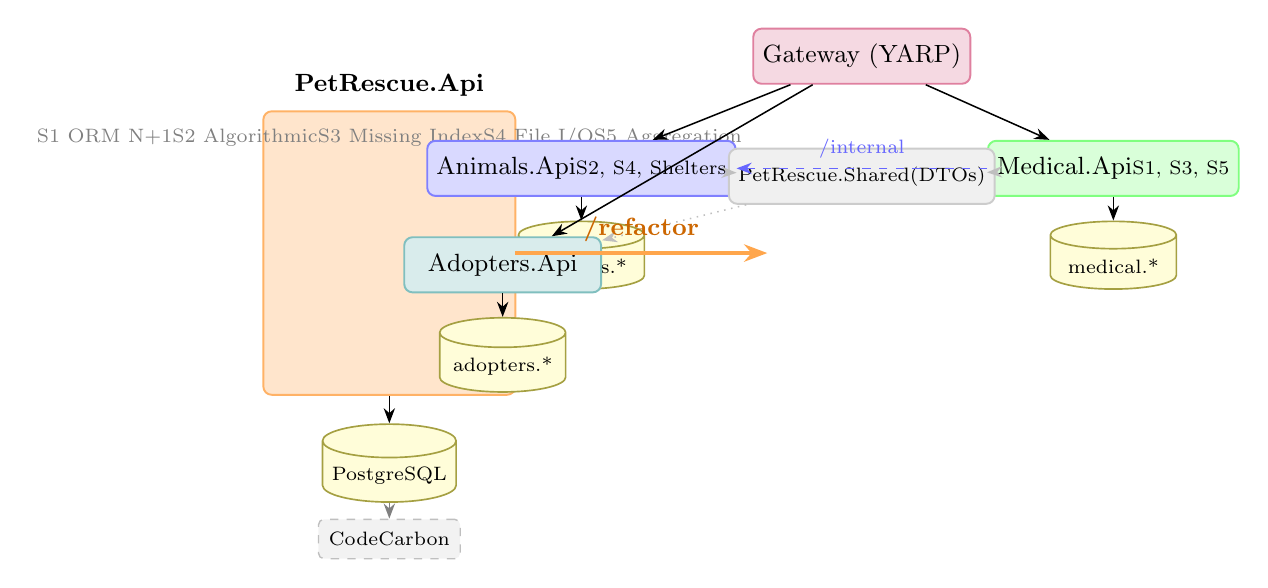
\begin{tikzpicture}[
  svc/.style   = {rectangle, rounded corners=3pt, minimum width=2.5cm,
                  minimum height=0.7cm, font=\small, text centered,
                  line width=0.7pt},
  db/.style    = {cylinder, shape border rotate=90, aspect=0.25,
                  minimum width=1.6cm, minimum height=0.55cm,
                  font=\scriptsize, text centered,
                  fill=yellow!15, draw=yellow!60!black, line width=0.6pt},
  sidecar/.style={rectangle, dashed, rounded corners=2pt,
                  minimum width=1.8cm, minimum height=0.5cm,
                  font=\scriptsize, text centered,
                  fill=gray!10, draw=gray!50, line width=0.5pt},
  arr/.style   = {-Stealth, line width=0.55pt},
  node distance= 0.4cm
]

% ===================== LEFT: MONOLITH =====================
\node[svc, fill=orange!20, draw=orange!60, minimum width=3.2cm,
      minimum height=3.6cm, align=center]
  (mono) at (-4,0) {};
\node[font=\small\bfseries, above=0.05cm of mono.north] {PetRescue.Api};
\node[font=\scriptsize, text=gray, below=0.1cm of mono.north, anchor=north]
  (s1lbl) {S1 ORM N+1\\S2 Algorithmic\\S3 Missing Index\\S4 File I/O\\S5 Aggregation};

\node[db, below=0.35cm of mono]
  (monodb) {PostgreSQL};
\draw[arr] (mono) -- (monodb);

\node[sidecar, below=0.2cm of monodb]
  (cc1) {CodeCarbon};
\draw[arr, dashed, gray] (monodb) -- (cc1);

% ===================== RIGHT: MICROSERVICES =====================
% Gateway
\node[svc, fill=purple!15, draw=purple!50,
      minimum width=2.6cm]
  (gw) at (2,2.5) {Gateway (YARP)};

% Animals.Api
\node[svc, fill=blue!15, draw=blue!50,
      below left=0.7cm and 0.2cm of gw]
  (animals) {Animals.Api\\{\scriptsize S2, S4, Shelters}};
\node[db, below=0.3cm of animals]
  (animalsdb) {animals.*};

% Medical.Api
\node[svc, fill=green!15, draw=green!50,
      below right=0.7cm and 0.2cm of gw]
  (medical) {Medical.Api\\{\scriptsize S1, S3, S5}};
\node[db, below=0.3cm of medical]
  (medicaldb) {medical.*};

% Adopters.Api
\node[svc, fill=teal!15, draw=teal!50,
      below=0.5cm of animals, xshift=-1.0cm]
  (adopters) {Adopters.Api};
\node[db, below=0.3cm of adopters]
  (adoptersdb) {adopters.*};

% Shared Contracts
\node[svc, fill=gray!12, draw=gray!40,
      below=0.8cm of gw, xshift=0cm, font=\scriptsize]
  (shared) {PetRescue.Shared\\(DTOs)};

% arrows: gateway → services
\draw[arr] (gw) -- (animals);
\draw[arr] (gw) -- (medical);
\draw[arr] (gw) -- (adopters);

% arrows: services → dbs
\draw[arr] (animals)  -- (animalsdb);
\draw[arr] (medical)  -- (medicaldb);
\draw[arr] (adopters) -- (adoptersdb);

% cross-service: Medical calls Animals /internal
\draw[arr, dashed, blue!60]
  (medical.west) -- node[above,font=\scriptsize,blue!60]{/internal} (animals.east);

% Shared contracts
\draw[arr, gray!50, dotted] (shared) -- (animals);
\draw[arr, gray!50, dotted] (shared) -- (medical);
\draw[arr, gray!50, dotted] (shared) -- (adopters);

% ===================== MIGRATION ARROW =====================
\draw[-Stealth, line width=1.2pt, orange!70]
  (-2.4, 0) -- node[above,font=\small\bfseries,orange!80!black]{/refactor} (0.8, 0);

\end{tikzpicture}

  \caption{The migration.  Slice~1 (monolith, left) is decomposed by
    \texttt{/refactor} into Slice~1~Refactored (right).
    Slice~2 (expert, not shown) is structurally identical to
    Slice~1~Refactored across all 20 dimensions in
    Table~\ref{tab:dimensions}.}
  \label{fig:arch}
\end{figure}

The most significant result is dimension~16: the loopback-only
\texttt{AddEndpointFilter} on the \texttt{/internal} endpoint group.
This security pattern was \emph{not} specified in the \texttt{/refactor}
skill prompt.  The expert author applied it because she recognised that
inter-service calls must never be reachable from the public internet;
the AI model inferred the same requirement from the absence of any
authentication middleware in Slice~1.  Both arrived at the same
defence independently.  Similarly, dimension~12--15: the exact shape
of the \texttt{AnimalsClient}—three endpoints, not one—was independently
chosen by both the expert and the AI to minimise network round-trips for
the S1 and S5 cross-context scenarios.
On elapsed time, the contrast is stark: the second author spent
approximately \textbf{one developer-day} designing and building
Slice~2; \texttt{/refactor} produced a structurally equivalent result
in approximately \textbf{five minutes}.  For a well-scoped .NET
monolith, the skill can substitute for a full boundary-analysis
session while producing a decomposition an experienced engineer would
recognise and trust.

\subsection{RQ2: Can the Pipeline Extend Both Codebases?}
We ran \texttt{/write\_code ShelterCapacity} on both
Slice~1~Refactored and Slice~2.  Reading only
\texttt{ARCHITECTURE.md}, the skill:
(a)~identified Animals.Api as the shelter-owning service;
(b)~added \texttt{ShelterCapacityDto} to the shared contracts library;
(c)~wrote a \texttt{ShelterCapacity.cs} handler with a server-side
SQL WHERE clause (no in-memory filtering);
(d)~registered the endpoint in \texttt{Program.cs}; and
(e)~added a YARP route in the gateway \texttt{appsettings.json}.

The two outputs were structurally identical.  The only differences
were namespace tokens and DTO field count (four in Slice~2, five in
Slice~1~Refactored—reflecting a \texttt{Status} field that
\texttt{/refactor} had inferred during the original migration).
Neither codebase required manual correction.
The complete quality-gated cycle—\texttt{/write\_code} through
\texttt{/publish}, including the \texttt{/review} and
\texttt{/check\_security} passes that surfaced and resolved security
findings—completed in approximately \textbf{30~minutes} on each
codebase.  This result validates the artefact-mediated state
principle: the skill required no knowledge of who wrote the codebase
or when—only the \texttt{ARCHITECTURE.md} contract was needed.

\subsection{RQ3: Does the Gate Prevent Unsafe Commits?}
Running \texttt{/check\_security} on Slice~2 reported three critical
findings:

\begin{itemize}
  \item \textbf{CRIT-01} — Hardcoded database credentials in all three
        \texttt{Program.cs} files.
  \item \textbf{CRIT-02} — Plain-text \texttt{POSTGRES\_PASSWORD} in
        \texttt{docker-compose.yml}.
  \item \textbf{CRIT-03} — Unauthenticated \texttt{/internal}
        endpoints on Animals.Api and Adopters.Api.
\end{itemize}

Four high-severity findings were also raised: inline Docker port
passwords, \texttt{AllowedHosts:~*} in all four
\texttt{appsettings.json} files, no HTTPS termination, and a
120-second HTTP client timeout.  \texttt{/fix} resolved all seven in
a single invocation and updated both gate documents to
\textsc{allowed}.  \texttt{/publish} then committed and pushed without
manual intervention.  Slice~1~Refactored presented the same finding
classes and was resolved identically.  Both repositories were
subsequently deployed to OCI via \texttt{terraform~apply}.

\begin{figure}[!t]
  \centering
  % Quality-gate cycle diagram
\begin{tikzpicture}[
  step/.style  = {rectangle, rounded corners=3pt, minimum width=2.4cm,
                  minimum height=0.65cm, font=\small\ttfamily,
                  text centered, line width=0.6pt},
  doc/.style   = {rectangle, rounded corners=2pt, minimum width=2.0cm,
                  minimum height=0.5cm, font=\scriptsize,
                  fill=gray!10, draw=gray!50, line width=0.4pt},
  decision/.style = {diamond, aspect=2.2, minimum width=2.8cm,
                     minimum height=0.8cm, font=\scriptsize,
                     fill=yellow!15, draw=yellow!60!black, line width=0.6pt},
  arr/.style   = {-Stealth, line width=0.6pt},
  block/.style = {arr, red!70},
  allow/.style = {arr, green!60!black},
  node distance = 0.45cm
]

% steps
\node[step, fill=blue!15, draw=blue!50]              (rv)   {/review};
\node[doc,  below=0.2cm of rv]                        (rvd)  {REVIEW.md};
\node[step, fill=blue!15, draw=blue!50,
      below=0.2cm of rvd]                             (sec)  {/check\_security};
\node[doc,  below=0.2cm of sec]                       (secd) {SECURITY.md};

\node[decision, below=0.35cm of secd]                 (gate) {any blocking\\or crit/high?};

% /fix branch (left)
\node[step, fill=red!15, draw=red!50,
      left=1.2cm of gate]                             (fix)  {/fix};

% /publish branch (right)
\node[step, fill=green!15, draw=green!50,
      right=1.2cm of gate]                            (pub)  {/publish};
\node[doc,  below=0.2cm of pub]                       (pubd) {git commit\\+ push};

% arrows
\draw[arr]    (rv)   -- (rvd);
\draw[arr]    (rvd)  -- (sec);
\draw[arr]    (sec)  -- (secd);
\draw[arr]    (secd) -- (gate);

\draw[block]  (gate) -- node[above,font=\scriptsize,red!70]{YES} (fix);
\draw[allow]  (gate) -- node[above,font=\scriptsize,green!60!black]{NO} (pub);
\draw[arr]    (pub)  -- (pubd);

% fix loops back up
\draw[arr, red!60, rounded corners=4pt]
  (fix.north) |- ([yshift=0.25cm]rv.north west) -- (rv.north west);

% fix patches docs
\draw[arr, red!60, dashed]
  (fix.east) to[bend right=20] node[right,font=\scriptsize,red!60]{patches} (secd.west);
\draw[arr, red!60, dashed]
  (fix.east) to[bend right=40] node[right,font=\scriptsize,red!60]{patches} (rvd.west);

% annotations
\node[font=\scriptsize, text=red!70, above=0.1cm of fix] {remediates\\blocking\\+ crit/high};
\node[font=\scriptsize, text=green!60!black, below=0.1cm of pubd]
  {clean\\repository};

\end{tikzpicture}

  \caption{The gated autonomy cycle, applied to both codebases.
    \texttt{/publish} is a hard precondition check: seven blocking and
    critical/high findings blocked the commit; \texttt{/fix}
    remediated all seven in a single pass; the gate cleared and
    \texttt{/publish} executed.  Medium/low findings remain visible
    for human review but do not block.}
  \label{fig:gate}
\end{figure}

% ============================================================
\section{Discussion}
\label{sec:discussion}
% ============================================================

\subsection{The Migration as a Complete Research Artefact}
The full migration—four public GitHub repositories, ten skill scripts,
JMeter load plans for five scenarios at three concurrency levels, a
CodeCarbon sidecar, and a Terraform configuration—constitutes a
self-contained, reproducible research artefact.  Any team can
clone Slice~1, run the ten skills in sequence, and arrive at a
deployed cloud service without modification.  This
end-to-end reproducibility distinguishes the work from migration case
studies that describe only the decomposition stage.

\subsection{What the 20/20 Match Tells Us About \texttt{/refactor}}
The convergence of the AI-generated and expert decompositions on all
twenty pre-defined dimensions is the strongest result in the paper.
It is stronger than a single-run benchmark because Slice~2 was
produced entirely independently—a different person, a different
toolchain, no communication with the pipeline.  The match is not
``the AI followed instructions well''; it is ``the AI and an expert
architect, working in isolation, made the same twenty decisions.''

The two uninstructed inferences (dimension~16: loopback protection;
dimensions~12--15: the three-endpoint AnimalsClient shape) are
especially significant.  They show that \texttt{/refactor} does not
merely translate requirements into scaffolding—it applies
domain-specific security and performance reasoning that the skill
prompt does not enumerate.  This points to a practical conclusion:
for a bounded .NET monolith with clear domain ownership, the
\texttt{/refactor} skill can substitute for a skilled architect in
the boundary-identification phase, the step practitioners report as
the hardest part of any migration~\cite{taibi2017processes}.

\subsection{Productivity Implications}
The elapsed-time data provide a concrete productivity signal.
The decomposition stage compressed from one developer-day to
approximately five minutes—a reduction that makes migration
\emph{exploratory} rather than \emph{committed}: a team can run
\texttt{/refactor} on a Monday, review the generated
\texttt{ARCHITECTURE.md} and service directories, and decide whether
to proceed before investing any manual effort.

The feature-addition cycle is equally instructive.  The 30-minute
end-to-end time \emph{includes} two quality-gate passes
(\texttt{/review} and \texttt{/check\_security}) that caught real
blocking and security findings.  A developer doing this manually
would either skip those checks—incurring security debt—or spend
substantially longer performing them.  The pipeline makes the
quality-assured path the \emph{fast} path, not the slow one.

These observations are consistent with findings on AI-assisted coding
productivity~\cite{peng2023copilot}, but extend them from single-file
completion to multi-service, security-gated, cloud-deployed workflows.

\subsection{Positioning Against Agentic SE Systems}
Existing agentic SE benchmarks~\cite{jimenez2024swebench} operate in
a continuous ReAct loop~\cite{yao2023react} and target single bug-fix
tasks.  Our pipeline extends the agentic paradigm in two directions:
workflow breadth (ten ordered, data-dependent stages versus a single
loop) and safety (explicit gate documents that block unsafe commits
versus a best-effort patch).  These are complementary dimensions;
loop-based agents could serve as the implementation engine inside
individual skills (e.g., \texttt{/fix}), while the gate architecture
governs the outer workflow.

\subsection{Practitioner Adoption Path}
Teams need not execute the full pipeline in one step.
The gate quartet (\texttt{/review} → \texttt{/check\_security} →
\texttt{/fix} → \texttt{/publish}) can be adopted as a commit-time
hygiene layer on any existing project immediately, without
\texttt{ARCHITECTURE.md} or any migration context.
\texttt{/write\_code} and the decomposition skills are additive once
an architecture document is in place.
The Terraform IaC layer is independent and can be paired with either
AI-generated or hand-crafted microservices, as demonstrated by
Slice~3 deploying both.

\subsection{Threats to Validity}
\textit{Internal validity.}  The twenty comparison dimensions were
derived from~\cite{taibi2017processes} and fixed before running
\texttt{/refactor}, but both authors know the codebase and may have
unconsciously biased the selection.  Slice~2 was completed before
\texttt{/refactor} was run, ruling out contamination.

\textit{External validity and reproducibility.}
We present this work explicitly as a \emph{reproducible pilot}.
The primary contribution is not the PetRescue migration result per se,
but the ten skill scripts that produced it.  Because every skill reads
from and writes to standard files (\texttt{ARCHITECTURE.md},
\texttt{REVIEW.md}, etc.), any team can clone the skill repository,
point it at their own .NET monolith, and replicate or refute the
findings on a different codebase without contacting the authors.
This distinguishes the work from a conventional case study: the
methodology is the artefact, and it is fully open.
Larger monoliths with circular bounded-context dependencies may yield
lower decomposition match scores; the gate and feature-addition skills
are largely scale-independent and are the strongest candidates for
adoption beyond .NET.

\textit{LLM non-determinism.}  Each skill was run once per codebase.
A multi-run study would quantify variance in the 20/20 result.

% ============================================================
\section{Conclusion}
\label{sec:conclusion}
% ============================================================

We have presented and evaluated a complete, end-to-end agentic AI
pipeline for migrating a .NET monolith to cloud-deployed microservices.
The pipeline's ten skills—grounded in the principles of skill
atomicity, artefact-mediated state, and gated autonomy—carry a
codebase from source analysis through decomposition, feature addition,
security remediation, gated commit, and Terraform deployment on an
OCI ARM64 instance.

The AI-generated migration matched an expert-crafted reference on all
twenty pre-defined structural dimensions.  A new feature was added
identically to both AI-generated and hand-crafted codebases using only
an \texttt{ARCHITECTURE.md} file as context.  Seven critical and
high-severity security findings were remediated without human
intervention; both repositories were published and deployed cleanly.

We present this as a \emph{reproducible pilot}: the ten skill scripts
are the reusable contribution, and PetRescue is the validation
vehicle.  Because every skill reads from and writes to plain Markdown
files, any team can apply the same pipeline to their own .NET monolith
and either replicate or extend the results without modification.
All four artefacts—Slice~1 (monolith), Slice~2 (expert
microservices), Slice~1~Refactored (AI microservices), and Slice~3
(Terraform IaC)—plus all ten skill scripts, are available at
\url{https://github.com/florinolariuip} for this purpose.

Future work will document community replications on open-source
.NET monoliths, measure the energy cost of AI-assisted migration
using the CodeCarbon sidecar, and quantify multi-run variance in
the decomposition agent.

% ============================================================
\section*{Acknowledgements}
The authors thank the reviewers for their constructive feedback.
% ============================================================

\balance
\bibliographystyle{IEEEtran}
\bibliography{references}

% ============================================================
%  AUTHOR BIOGRAPHIES
% ============================================================
\begin{IEEEbiography}[{\includegraphics[width=1in,height=1.25in,clip,keepaspectratio]{figures/florin-photo}}]
{Florin Olariu}
is a software engineer at Suvoda LLC and a researcher at the Faculty
of Computer Science, Alexandru Ioan Cuza University of Ia\c{s}i,
Romania.  His research interests include cloud-native architectures,
agentic AI for software engineering, and performance engineering.
He is a member of IEEE.
\end{IEEEbiography}

\begin{IEEEbiography}[{\includegraphics[width=1in,height=1.25in,clip,keepaspectratio]{figures/lenuta-photo}}]
{Lenuta Alboaie}
is an Associate Professor at the Faculty of Computer Science, Alexandru
Ioan Cuza University of Ia\c{s}i, Romania.  Her research interests
include distributed systems, cloud computing, and software
architectures.  She is a senior member of IEEE.
\end{IEEEbiography}

\end{document}
